\section{Generalized VPN problem}
To describe the generalized VPN problem, we first describe the class of tree demands.
Let $G = (V_G, E_G)$ be the underlying network graph with terminal set $W \subseteq V_G$.
Let an edge-capacitated tree $T = (V_T, E_T)$ be given with leaf set exactly the terminals $W$, and edge capacities $b_e$ for $e \in E_T$.
Then $T$ describes the tree demand universe $\mathcal U_T$ where a symmetric demand matrix $(D_{ij})$ belongs to $\mathcal U_T$ when it can be routed on $T$.
That is, for all edges $e$ on the (unique) path $\pi_T(i,j)$ between $i$ and $j$ in $T$ it must hold that $D_{ij} \le b_e$.
Note that if we take $T$ to be a star with center $r$ and edge capacities $b_{ir} = b_i$, then $\mathcal U_T$ describes the same universe as the hose model $\mathcal H$ with marginal demands $b_i$.
Hence, tree demands indeed generalize the hose model.

The generalized VPN is now fully characterized by the underlying network graph $G$, a terminal set $W$, edge per-unit-capacity costs $c_e$ ($e \in E_G$), and the \emph{demand tree} $T$ with edge capacities $b_f$ ($f \in E_T$).
A solution to the problem consists of a routing template $\mathcal P = \set{P_{ij} : i,j \in \binom W 2}$ and bought edge capacities $x_e$ for all $e \in E_G$.
We call a solution \emph{feasible} when all demand matrices in $\mathcal U_T$ can be routed on $G$ according to the routing template and without exceeding the installed edge capacities $x$.
We furthermore call a solution optimal if it is feasible and minimizes $\sum_{e \in E_G} c_e x_e$.

\subsection{Integer programming formulation}
The generalized VPN problem can be formulated as the integer program~\eqref{eq:gvpn:mip:semiinf:obj}--\eqref{eq:gvpn:mip:semiinf:f}.
\begin{alignat}{5}
    \text{minimize}\ && \sum_{uv \in E_G} c_{uv} \cdot x_{uv} &&& \label{eq:gvpn:mip:semiinf:obj}\\
    \text{subject to}\ && x_{uv} &\ge \sum_{ij \in \binom{W}{2}} D_{ij} \cdot (f_{uv}^{ij} + f_{vu}^{ij}) &&\qquad \forall_{uv \in E_G,\ D \in \mathcal U_T} \label{eq:gvpn:mip:semiinf:demand}\\
    && \sum_{uv \in \delta(u)} (f_{uv}^{ij} - f_{vu}^{ij}) &= \begin{cases}
                                                                  1 & \text{if $u = i$} \\
                                                                  -1 & \text{if $u = j$} \\
                                                                  0 & \text{otherwise}
    \end{cases} &&\qquad \forall_{u \in V_G,\ ij \in \binom{W}{2}} \label{eq:gvpn:mip:semiinf:flow}\\
    && x_{uv} &\in \mathbb{R}_+ &&\qquad \forall_{uv \in E_G} \label{eq:gvpn:mip:semiinf:x}\\
    && f_{uv}^{ij},\ f_{vu}^{ij} &\in \{ 0, 1 \} &&\qquad \forall_{uv \in E_G,\ ij \in \binom{W}{2}} \label{eq:gvpn:mip:semiinf:f}
\end{alignat}
Each edge $uv$ has constant cost $c_{uv}$ and has a non-negative variable $x_{uv}$ indicating the bought capacity for this edge.
The objective is then to minimize the total cost, i.e.\ the sum of $c_{uv} x_{uv}$ over all edges $uv$.

For each unordered pair of terminals $\set{i, j} \in \binom W 2$, a routing path between these terminals is constructed using binary flow variables.
The flow variable $f_{uv}^{ij}$ indicates whether the directed edge $(u, v)$ is used on the path from terminal $i$ to $j$.
This can be modeled with traditional flow constraints in constraint~\eqref{eq:gvpn:mip:semiinf:flow}.
The routing path from $i$ to $j$ is then given by the set of directed edges $\set{(u, v) \in E_G | f_{uv}^{ij} = 1}$.
By symmetry, we only need to consider one ordering of all unordered pairs.
For ease of notation, we will still describe flow variables with $f_{uv}^{ij}$.

Constraint~\eqref{eq:gvpn:mip:semiinf:demand} ensures that we buy enough capacity on each edge.
For a demand matrix $D \in \mathcal U_T$, we can derive the required capacity on an edge $uv$ using the flow variables.
If $f^{ij}_{uv}$ or $f^{ij}_{vu}$ is 1, then we must buy $D_{ij}$ capacity on edge $uv$ to facilitate the flow between terminals $i$ and $j$.
Thus, we obtain the constraint
\[
    x_{uv} \ge \sum_{ij \in \binom W 2} D_{ij} ( f^{ij}_{uv} + f^{ij}_{vu}),
\]
which must hold for any edge $uv$ and for any demand matrix $D_{ij} \in \mathcal U_T$.

This definition leads to an infinite number of constraints as $\mathcal U_T$ is in general not a finite set of matrices.
This issue can be resolved with row generation, where we solve the program by only considering a subset $\mathcal U_T^* \subset \mathcal U_T$ in constraint~\eqref{eq:gvpn:mip:semiinf:demand}.
Then we obtain a solution $(\tilde x, \tilde f)$ that is only valid for all $D \in \mathcal U_T^*$.
We then assess whether there exists a matrix $D \in \mathcal U_T \setminus \mathcal U_T^*$ that violates the constraint.
If such a matrix exists, we add it to $\mathcal U_T^*$ and solve the program again until we cannot find any violating matrix.
Note that a violating matrix $D$ satisfies
\[
    \tilde x_{uv} < \sum_{ij \in \binom W 2} D_{ij} \cdot (\tilde f^{ij}_{uv} + \tilde f^{ij}_{vu})
\]
for some edge $uv \in E_G$.
We can thus find such a violating matrix by solving the following linear subproblems, one for each $uv \in E_G$:
\begin{alignat*}{5}
    p_{uv} = \text{maximize}\quad && \sum_{ij \in \binom{W}{2}} (\tilde f_{uv}^{ij} + \tilde f_{vu}^{ij}) \cdot D_{ij} &&& \\
    \text{subject to}\quad && \sum_{\substack{ij \in \binom{W}{2}\\e \in \pi_T(i,j)}} D_{ij} &\le b_e &&\qquad \forall_{e \in E_T} \\
    && D_{ij} &\in \mathbb{R}_+ &&\qquad \forall_{ij \in \binom{W}{2}}
\end{alignat*}
If for any of these subproblems the optimal solution $D^*$ has objective $p_{uv} > \tilde x_{uv}$, we add $D^*$ to $\mathcal U_T^*$.
Otherwise, $\mathcal U_T^*$ was representative for $\mathcal U_T$ and we can conclude that the integer program~\eqref{eq:gvpn:mip:semiinf:obj}--\eqref{eq:gvpn:mip:semiinf:f} is optimal.

Although the row generation subproblems do not contain integer variables, the overall procedure to find an optimal solution for \eqref{eq:gvpn:mip:semiinf:obj}--\eqref{eq:gvpn:mip:semiinf:f} may use a large number of iterations.
Using a clever dualization trick (also performed in~\cite{altin2007provisioning}) we can obtain a compact MIP formulation that does not require row generation.

For this trick, consider a single edge $uv \in E_G$ and consider $f$ as parameters.
Note that we can write constraint~\ref{eq:gvpn:mip:semiinf:demand} as
\[
    x_{uv} \ge \max_{D \in \mathcal U_T} \sum_{ij \in \binom W 2} D_{ij} \cdot (f^{ij}_{uv} + f^{ij}_{vu}),
\]
or, when writing out the polyhedral constraints describing $\mathcal U_T$, as the optimization problem
\begin{alignat}{5}
    x_{uv} \ge \text{maximize}\ && \sum_{ij \in \binom{W}{2}} (f_{uv}^{ij} + f_{vu}^{ij}) \cdot D_{ij} &&& \\
    \text{subject to}\ && \sum_{\substack{ij \in \binom{W}{2}\\e \in \pi_T(i,j)}} D_{ij} &\le b_e &&\qquad \forall_{e \in E_T} \label{eq:gvpn:dualtrick} \\
    && D_{ij} &\in \mathbb{R}_+ &&\qquad \forall_{ij \in \binom{W}{2}}
\end{alignat}
Since this linear program is feasible and bounded, we might just as well write the dual
\begin{alignat}{5}
    x_{uv} \ge \text{minimize}\ && \sum_{e \in E_T} b_e \cdot \omega_e^{uv} &&& \label{eq:gvpn:dualtrick:min} \\
    \text{subject to}\ && \sum_{e \in \pi_T(i,j)} \omega_e^{uv} &\ge f_{uv}^{ij} + f_{vu}^{ij} &&\qquad \forall_{ij \in \binom{W}{2}} \\
    && \omega_e^{uv} &\in \mathbb{R}_+ &&\qquad \forall_{e \in E_T}
\end{alignat}
where $\omega_e^{uv}$ are the  dual variables for constraint~\ref{eq:gvpn:dualtrick}.
Now, note that we can drop the minimize in \ref{eq:gvpn:dualtrick:min} as the objective function of the original MIP is a non-negatively weighted sum of the variables $x_{uv}$.
We now have thus obtained a compact MIP formulation for the generalized VPN problem:
\begin{alignat*}{5}
    \text{minimize}\ && \sum_{uv \in E_G} c_{uv} \cdot x_{uv} &&& \\
    \text{subject to}\ && x_{uv} &\ge \sum_{e \in E_T} b_e \cdot \omega_e^{uv} &&\qquad \forall_{uv \in E_G} \\
    && \sum_{e \in \pi_T(i,j)} \omega_e^{uv} &\ge f_{uv}^{ij} + f_{vu}^{ij} &&\qquad \forall_{uv \in E_G,\ ij \in \binom{W}{2}} \\
    && \sum_{uv \in \delta(u)} (f_{uv}^{ij} - f_{vu}^{ij}) &= \begin{cases}
                                                                1 & \text{if $u = i$} \\
                                                                -1 & \text{if $u = j$} \\
                                                                0 & \text{otherwise}
    \end{cases} &&\qquad \forall_{u \in V_G,\ ij \in \binom{W}{2}} \\
    && x_{uv} &\in \mathbb{R}_+ &&\qquad \forall_{uv \in E_G} \\
    && \omega_e^{uv} &\in \mathbb{R}_+ &&\qquad \forall_{uv \in E_G,\ e \in E_T} \\
    && f_{uv}^{ij},\ f_{vu}^{ij} &\in \{ 0, 1 \} &&\qquad \forall_{uv \in E_G,\ ij \in \binom{W}{2}}
\end{alignat*}

\subsection{Hierarchical hubbing algorithm}
\begin{algorithm}
    \caption{RecursiveHubbing}
    \label{alg:TriangulateStar}
    \begin{algorithmic}[1]
        \Statex Recursive enumeration algorithm to find all optimal mappings. Initially, verticesToAssign equals $V_T - W$ and $h$ is an empty mapping from $V_T$ to $V_G$. In the actual implementation, we also maintain a set of all best mappings that attain the minimum cost.

        \Procedure{Assign}{verticesToAssign, $h$}
            \If {verticesToAssign is empty}
                \State \Return $\sum_{uv \in E_T} d(h(u), h(v))$ \Comment{The cost of mapping $h$}
            \EndIf

            \State $u \gets$ verticesToAssign.first()
            \State bestCost $\gets \infty$

            \ForAll {vertices $v$ in graph}
                \State $h(u) \gets v$
                \State currentCost $\gets$ \textsc{Assign}(verticesToAssign $-$ $u$, $h$)

                \If {currentCost $<$ bestCost}
                    \State bestCost $\gets$ currentCost
                \EndIf
            \EndFor

            \State \Return bestCost
        \EndProcedure
    \end{algorithmic}
\end{algorithm}

Olver and Shepherd suggested an 8-approximation algorithm for this problem~\cite{olver2010approxrnd}.
They considered the optimal solution over all \emph{hubbing solutions}.
A hubbing solution maps each internal node in the demand tree to a vertex in $V_G$.
Each terminal must be mapped to its corresponding vertex in $G$.
This mapping function is denoted with $h$
For each edge $uv$ in the demand tree, we then buy $b_{uv}$ capacity along the shortest path between $h(u)$ and $h(v)$ in the original graph $G$, where each edge $e$ has its cost $c_e$ as weight.
The total cost then becomes
\[
    \sum_{uv \in E_T} b_{uv} d_c(h(u), h(v)),
\]
where $d_c(h(u), h(v))$ gives the distance between $h(u)$ and $h(v)$ in $G$ where $c$ defines the edge weights.
It was conjectured that this algorithm is optimal, i.e.\ that an optimal hubbing solution is an optimal solution for the generalized VPN problem.

Algorithm~\ref{alg:TriangulateStar} describes a recursive algorithm to find the optimal hubbing solution.
With a standard recursive approach, the total cost is calculated for each mapping $h$ from $V_T \setminus W$ to $V_G$.
The optimal cost is then returned; notice that the actual mapping can easily be returned as well.
From this mapping, the routing templates can be derived.

However, it is possible to determine the optimal hubbing solution more efficiently using dynamic programming~\cite{olver2010approxrnd}.
We first pick an arbitrary internal node of the demand tree as root.
Then we root the demand tree here.
A subtree of this tree is a tree that is rooted at a vertex in this tree, i.e.\ a vertex and all nodes below it.
This tree has a parent (unless it is the entire tree) and children (unless the root is a terminal).
Algorithm~\ref{alg:subtrees} derives the set of subtrees, denoted by $\mathcal L$, in a BFS manner.

For any subtree $S \in \mathcal L$ and vertex $v \in V_G$, we consider the subproblem $C[S, v]$.
It stores the cost of an optimal hubbing solution of the problem restricted to subtree $S$, where the root of $S$ is mapped to $v$.
The final solution is then $\min_{v \in V_G} C[T, v]$.

Let $S_w$ denote the subtree rooted at a vertex $w \in T$.
Now suppose that we want to obtain the value for $C[S_r, v]$ for some vertex $r \in V_T$ and $v \in V_G$, while $C[S_{r_i}, w]$ is known for all children $r_i$ of $r$ and all vertices $w \in V_G$.
Then the mappings of the subtrees are independent of each other.
The contribution of one specific subtree $S_{r_i}$ to the cost of subtree $S_r$ is
\[
    \min_{w \in V_G} \left( C[S_{r_i}, w] + b_{r, r_i} d_c(v, w) \right).
\]
Notice that the mapping of $r$ is $v$ and the mapping of $r_i$ is $w$ in this recurrence.
We minimize the cost of this subtree over all possible choices for $w$.
This gives the following recurrence.
\[
    C[S_r, v] = \begin{cases}
                  0 &\text{if $r \in W$ and $r = v$} \\
                  \infty &\text{if $r \in W$ and $r \neq v$} \\
                  \displaystyle \sum_{\text{children $r_i$ of $r$}} \min_{w \in V_G} \Big( C[S_{r_i}, w] + b_{r, r_i} d(v, w) \Big) &\text{otherwise} \\
    \end{cases}
\]

\begin{algorithm}
    \caption{Finding all subtrees for the dynamic programming algorithm}
    \label{alg:subtrees}
    \begin{algorithmic}[1]
        \Statex Obtaining all subtrees that are needed for the dynamic programming algorithm.
        The dynamic program itself only fills in the table based on the recurrence stated below.
        \Procedure{GetSubtrees}{$V_T, E_T, W$}
            \State root = arbitrary node in $V_T - W$

            \State $\mathcal L \gets \emptyset$
            \State $S \gets$ Subtree(root, root.neighbors, null) \Comment{A subtree has a root, children and parent}
            \State $\mathcal L$.add($S$)
            \State $\mathcal Q$.add($S$)

            \While {$\mathcal Q$ is not empty}
                \State tree $\gets \mathcal Q$.removeFirst()
                \State currentRoot $\gets$ tree.root
                \ForAll{vertices $r$ in tree.children}
                    \State $S$ = Subtree($r$, $r$.neighbors $-$ currentRoot, currentRoot)
                    \State $\mathcal L$.add($S$)
                    \State $\mathcal Q$.add($S$)
                \EndFor
            \EndWhile
            \State \Return subtrees.reversed()
        \EndProcedure
    \end{algorithmic}
\end{algorithm}

\subsection{Experiments}
All the experiments we have seen.
Integrality gap results.

\subsection{Proving the generalized VPN conjecture on ring networks}
The paper by Grandoni et al.~\cite{grandoni2008short} gives a short proof that the VPN conjecture is true for the cases where $G$ is a ring.
In this section, we will discuss an attempt to extend the proof to the generalized VPN conjecture, for the cases where the network is a ring and the demand tree is a \emph{two-union star}: the tree formed by connecting the centers of two star graphs.
We refer to this edge between the centers as the bridge.

As mentioned in \cite{grandoni2008short}, the hubbing solution that is computed by the polynomial-time algorithm is also a \emph{tree solution}, that is, the support of the routing template forms a tree.
Exploiting this structure is key for the argument to work.
In the generalized setting however, the hierarchical hubbing solution may not be a tree solution, even in the restricted case of the ring network with a two-union star demand tree.
A small counterexample is given in Figure~\ref{fig:counterex-tree-solution}.
In any optimal hubbing solution, the internal node $R^+$ needs to be mapped to either to the site of $B^+$ or $C^+$ in $G$.
Symmetrically, $R^-$ needs to be mapped to either $B^-$ or $C^-$.
The optimal hubbing solution is then no tree solution, as the shortest path between the mapped $R^+$ and $R^-$ uses the bottom edge between $C^+$ and $C^-$, while the shortest path between the mapped $R^+$ and $A^+$ goes via $A^-$, and likewise the shortest path between the mapped $R^-$ to $A^-$ goes via $A^+$.
Indeed, the support of the routing template is the whole cycle $G$.

\begin{figure}
    \centering
    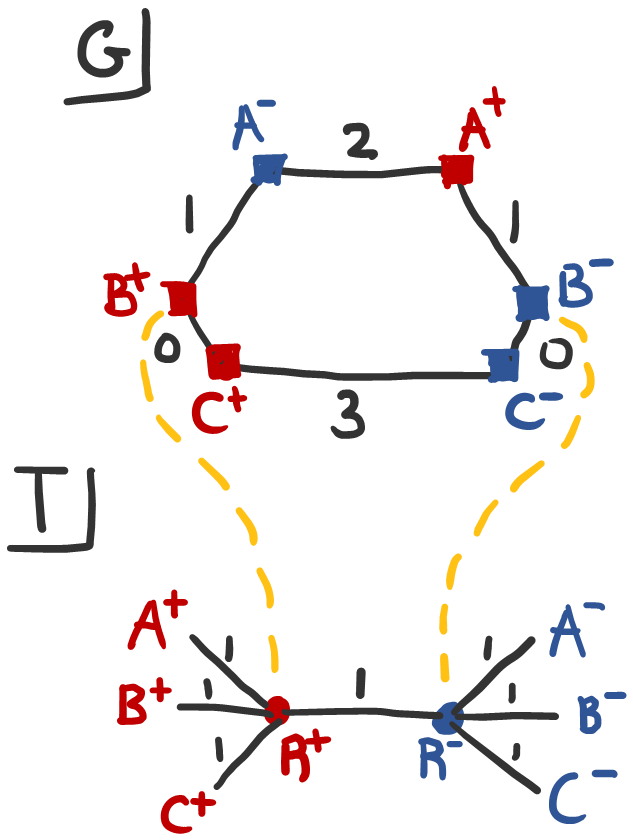
\includegraphics[width=.3\textwidth]{counterexample-tree-solution}
    \caption{Counterexample that the optimal hubbing solution is a tree solution.} \label{fig:counterex-tree-solution}
\end{figure}

The above counterexample uses a demand tree with (at least) three terminals at either side of the two-union star, and one might wonder what happens for the case where there are only two terminals on one side (notice that the case is solved when having only one terminal, as then the demand tree reduces to a star).
With a slightly different construction as in Figure~\ref{fig:counterex2}, we see that no tree solution is guaranteed here either. % TODO: explanation

\begin{figure}
    \centering
    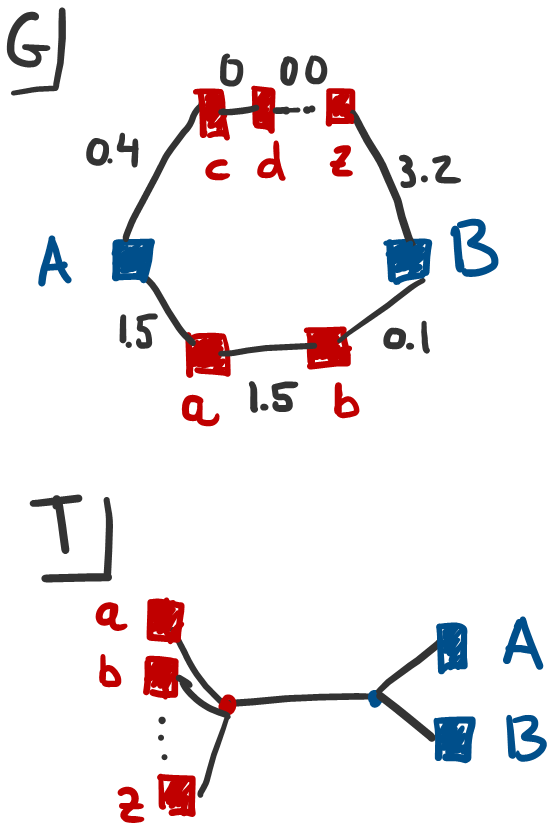
\includegraphics[width=.3\textwidth]{counterexample2}
    \caption{Counterexample that the optimal hubbing solution is a tree solution, when one side of the demand tree has only two terminals.}
    \label{fig:counterex2}
\end{figure}

% TODO: move to appendix?
Some background of what steps we are taking is identical to what is described in \cite{grandoni2008short} and we will omit these details.
We focus on showing the differences that are necessary in the proof to adapt to the generalized VPN problem setting.
We use the same notation as used in the aforementioned paper, except where the generalized VPN problem differs from the VPN problem.

For the remainder, we restrict ourselves to instances where $T$ is a \emph{two-union star}, that is, a tree formed by connecting the centers $r_1,\ r_2$ of two star graphs.
We will call this edge $r = \set{r_1, r_2}$ and refer to it as the \emph{bridge} of $T$.

\subsubsection{Preliminaries}
A number of assumptions are made in \cite{grandoni2008short}, the most important being that we can assume the capacities $b \equiv 1$.
We suspect this does not quite generalize to our case, but we can state the following:

\begin{fact}
    We may assume $b_f = 1$ when $f \neq r$.
\end{fact}
Using the same motivation as in \cite{grandoni2008short}, if the capacity $b_{iu}$ for a terminal $i \in W$ is not unit, construct a new instance with new terminals $i_1, \dots, i_{b_{iu}}$, connected to the site of $i$ in $G$, with edge cost $0$.
Set the capacities of the incident edges in $T$ to unit.
Note that this instance is equivalent, but may change the topology of the graph.

An alternative construction is argued in \cite{grandoni2008short} to keep the topology a ring and we refer to this paper for the details.

\begin{fact}
    We can assume $b$ to be integral.
\end{fact}
This is motivated by scaling by a sufficiently large factor.

\subsubsection{Pyramidal Routing problem}
To goal is to show that there exists an optimal solution to the generalized VPN problem that is a tree solution (or, equivalently, there exists a tree solution to the generalized VPN problem that is optimal).
Consider an optimal tree solution $(\set{P_{ij}}, u)$ to a generalized VPN instance $(G, c, W, T, b)$, with $|W| = k$ and $T$ a two-union star with the unit capacity assumption as above.
Let $\mathcal P_i$ be as in \cite{grandoni2008short} for a fixed $i \in W$.
We define
\[
    \xi(e, \mathcal P_i) \coloneqq \min\set{\alpha(e, \mathcal P_i),\ \beta(e, \mathcal P_i)} + \min\set{n(e, \mathcal P_i) - \alpha(e, \mathcal P_i),\ k - n(e, \mathcal P_i) - \beta(e, \mathcal P_i)}
\]
where
\begin{gather*}
    n(e, \mathcal P_i) \coloneqq |\set{j \in W \setminus \set{i} : e \in P_{ij}}|,\\
    \alpha(e, \mathcal P_i) \coloneqq |\set{j \in W \setminus \set{i} : e \in P_{ij},\ r \in \pi_T(i, j)}|,\\
    \beta(e, \mathcal P_i) \coloneqq |\set{j \in W \setminus \set{i} : e \not\in P_{ij},\ r \not\in \pi_T(i, j)}|,
\end{gather*}
that is, $\alpha(e, \mathcal P_i)$ is the number of paths in $\mathcal P_i$ containing $e$, \emph{while simultaneously the path in the demand tree between $i$ and $j$ crosses the bridge}.
In our setting, we have a different expression for the \emph{required} capacity of edge $e$:
\[
    u(e) = \xi(e, \mathcal P_i) + \min\Big\{b(r),\ n(e, \mathcal P_i) - \xi(e, \mathcal P_i),\ k - n(e, \mathcal P_i) -  \xi(e, \mathcal P_i)\Big\}.
\]
We can now formulate the generalized Pyramidal Routing (\emph{genPR}) problem with instance $(G, c, W, T, b, i)$ as to minimize $\sum_{e \in E_G} c(e) y(e, \mathcal P_i)$ over all $\mathcal P_i$ (for an arbitrary fixed $i \in W$), where we define
\[
    y(e, \mathcal P_i) = \xi(e, \mathcal P_i) + \min\Big\{b(r),\ n(e, \mathcal P_i) - \xi(e, \mathcal P_i),\ k - n(e, \mathcal P_i) -  \xi(e, \mathcal P_i)\Big\}.
\]

We now formulate our version of Conjecture~2 (as in \cite{grandoni2008short}).
\renewcommand\theconjecture{2}
\begin{conjecture}[The \emph{genPR} conjecture]
    For each \emph{genPR} instance $(G, C, W, i, T, b)$ there exists an optimal solution which is a tree solution.
\end{conjecture}

We now show our version of Theorem~1 (having the same formulation as in \cite{grandoni2008short}), using the equivalent of Lemma~3, Claim~1, and Claim~2.

\renewcommand\thelemma{3}
\begin{lemma}
    Consider an generalized VPN instance $(G, c, W, T, b)$ with $T$ a two-union star with bridge $r$, $b(f) = 1$ for $f \neq r$, and some feasible solution $(\set{P_{ij}}, u)$.
    There exists a terminal $i \in W$ such that $\sum_{e \in E_G} c(e) u(e) \ge \sum_{e \in E_G} c(e) y(e, \mathcal P_i)$, where $\mathcal P_i = \set{P_{ij} : j \in W \setminus \set{i}}$.
\end{lemma}
\begin{proof}
    Fix an edge $e \in E_G$.
    We define the same traffic matrix $D^e = (d^e_{ij})_{i,j \in W}$ as in \cite{grandoni2008short},
    \[
        d^e_{ij} = \begin{cases}
                       \frac 1 k \left( \frac{y(e, \mathcal P_i)}{n(e, \mathcal P_i)} + \frac{y(e, \mathcal P_j)}{n(e, \mathcal P_j)} \right) & \text{if $e \in P_{ij}$,} \\
                       0 & \text{otherwise.}
        \end{cases}
    \]

    Now, the proof of Claim~1 is slightly different, as our universe is described by a different set of inequalities.

    \renewcommand\theclaim{1}
    \begin{claim}
        $D^e \in \mathcal U_T$, that is
        \[
            \sum_{\substack{ij \in \binom{W}{2}:\\f \in \pi_T(i,j)}} d^e_{ij} \le b(f)
        \]
        for all $f \in E_T$.
    \end{claim}
    \begin{proof}
        We consider two cases:
        \begin{itemize}
            \item $f \neq r$, hence we can write $f = f_i$, where $f_i \in E_T$ is the edge incident some terminal $i \in W$.
            Now note that we can write
            \[
                \sum_{\substack{\ell j \in \binom{W}{2}:\\f_i \in \pi_T(\ell,j)}} d^e_{\ell j} = \sum_{j \in W \setminus \set{i}} d^e_{ij}
            \]
            as $f_i$ is exactly in all paths from/to $i$ in the tree, as it is the edge incident to $i$.
            The rest of this case follows the same steps as the proof in \cite{grandoni2008short}:
            \[
                \begin{split}
                    \sum_{\substack{\ell j \in \binom{W}{2}:\\f_i \in \pi_T(\ell,j)}} d^e_{\ell j} &= \sum_{j \in W \setminus \set{i}} d^e_{ij} \\
                    &= \frac 1 k \sum_{\substack{j \in W \setminus \set{i}:\\ e \in P_{ij}}} \left( \frac{y(e, \mathcal P_i)}{n(e, \mathcal P_i)} + \frac{y(e, \mathcal P_j)}{n(e, \mathcal P_j)} \right) \\
                    &\le \frac 1 k \sum_{\substack{j \in W \setminus \set{i}:\\ e \in P_{ij}}} \left( \frac{k - n(e, \mathcal P_i)}{n(e, \mathcal P_i)} + \frac{n(e, \mathcal P_j)}{n(e, \mathcal P_j)} \right) \\
                    &= \frac{1}{n(e, \mathcal P_i)} \sum_{\substack{j \in W \setminus \set{i}:\\ e \in P_{ij}}} 1 \\
                    &= 1 \\
                    &= b(f_i).
                \end{split}
            \]

            \item $f = r$.
            We have not been able, with the current definition of $y$ and $D^e$, to make this work.
            However, we reduced it to a more accessible form.
            In the third line, we exchange the order of the two sums and use the symmetry of $\pi_T(i, j)$ and $P_{ij}$.
            \[
                \begin{split}
                    \sum_{\substack{ij \in \binom{W}{2},\\r \in \pi_T(i,j)}} d^e_{ij} &= \frac 1 2 \sum_{i \in W} \sum_{\substack{j \in W \setminus \set{i}:\\r \in \pi_T(i,j)}} d^e_{ij} \\
                    &= \frac{1}{2k} \sum_{i \in W} \sum_{\substack{j \in W \setminus \set{i}:\\r \in \pi_T(i,j),\\e \in P_{ij}}} \frac{y(e, \mathcal P_i)}{n(e, \mathcal P_i)} + \frac{1}{2k} \sum_{i \in W} \sum_{\substack{j \in W \setminus \set{i}:\\r \in \pi_T(i,j),\\e \in P_{ij}}} \frac{y(e, \mathcal P_j)}{n(e, \mathcal P_j)} \\
                    &= \frac{1}{2k} \sum_{i \in W} \sum_{\substack{j \in W \setminus \set{i}:\\r \in \pi_T(i,j),\\e \in P_{ij}}} \frac{y(e, \mathcal P_i)}{n(e, \mathcal P_i)} + \frac{1}{2k} \sum_{j \in W} \sum_{\substack{i \in W \setminus \set{j}:\\r \in \pi_T(j,i),\\e \in P_{ji}}} \frac{y(e, \mathcal P_j)}{n(e, \mathcal P_j)} \\
                    &= \frac{1}{k} \sum_{i \in W} \sum_{\substack{j \in W \setminus \set{i}:\\r \in \pi_T(i,j),\\e \in P_{ij}}} \frac{y(e, \mathcal P_i)}{n(e, \mathcal P_i)} \\
                    &= \frac{1}{k} \sum_{\substack{i \in W:\\n(e, \mathcal P_i) > 0}} \left( \alpha(e, \mathcal P_i) \frac{y(e, \mathcal P_i)}{n(e, \mathcal P_i)} \right) \\
                    &\ \vdots\\
                    &\le b(r).
                \end{split}
            \] \qedhere
        \end{itemize}

    \end{proof}
    The remainder of the proof of Lemma~3 (and Claim~2) is exactly the same as in \cite{grandoni2008short}, as the definition of $D^e$ is exactly the same, and the definition of $y(e, \mathcal P_i)$ itself is not used.
\end{proof}

From this follows (our version of) Theorem~1, stating that on ring networks, if there exists an optimal tree solution for the \emph{genPR} problem, that also an optimal tree solution exists for the generalized VPN problem.

Now, what remains to show is that indeed an optimal tree solution exists for the \emph{genPR} problem when $G$ is a ring.
If we follow the structure of the proof in \cite{grandoni2008short}, not first that Claim~3 also holds for our case.
However, Claim~4 does not hold: it might be that $y(e, \mathcal P_i) = y(f, \mathcal P_i) = b(r)$ (in the second case of the definition of $y$).
We have not quite yet mastered the inductive proof that follows (in which Claim~4) is used.
Therefore, we are not sure that the counterexample for Claim~4 is actually problematic, or how to circumvent this issue.
